% !TEX program = pdflatex
\documentclass[a4paper,14pt]{extarticle}

% ===== Язык и кодировка (pdfLaTeX, Overleaf) =====
\usepackage[T2A]{fontenc}
\usepackage[utf8]{inputenc}
\usepackage[russian,english]{babel}

% ===== Поля =====
\usepackage[left=30mm, right=15mm, top=20mm, bottom=20mm]{geometry}

% ===== Графика и таблицы =====
\usepackage{graphicx}
\usepackage{longtable}
\usepackage{array}
\usepackage{booktabs}
\usepackage{float}

% ===== Листинги кода и Verbatim =====
\usepackage{listings}
\usepackage{xcolor}
\usepackage{fancyvrb}

\lstset{
  language=Python,
  basicstyle=\footnotesize\ttfamily,
  keywordstyle=\color{blue}\bfseries,
  commentstyle=\color{gray}\itshape,
  stringstyle=\color{red!70!black},
  numbers=left,
  numberstyle=\tiny\color{gray},
  numbersep=8pt,
  frame=single,
  breaklines=true,
  breakatwhitespace=false,
  tabsize=4,
  showstringspaces=false,
  captionpos=b,
  extendedchars=true,
  inputencoding=utf8,
  literate=
    {а}{{\cyra}}1  {б}{{\cyrb}}1  {в}{{\cyrv}}1  {г}{{\cyrg}}1
    {д}{{\cyrd}}1  {е}{{\cyre}}1  {ё}{{\cyryo}}1 {ж}{{\cyrzh}}1
    {з}{{\cyrz}}1  {и}{{\cyri}}1  {й}{{\cyrishrt}}1 {к}{{\cyrk}}1
    {л}{{\cyrl}}1  {м}{{\cyrm}}1  {н}{{\cyrn}}1  {о}{{\cyro}}1
    {п}{{\cyrp}}1  {р}{{\cyrr}}1  {с}{{\cyrs}}1  {т}{{\cyrt}}1
    {у}{{\cyru}}1  {ф}{{\cyrf}}1  {х}{{\cyrh}}1  {ц}{{\cyrc}}1
    {ч}{{\cyrch}}1 {ш}{{\cyrsh}}1 {щ}{{\cyrshch}}1 {ъ}{{\cyrhrdsn}}1
    {ы}{{\cyrery}}1 {ь}{{\cyrsftsn}}1 {э}{{\cyrerev}}1 {ю}{{\cyryu}}1
    {я}{{\cyrya}}1
    {А}{{\CYRA}}1  {Б}{{\CYRB}}1  {В}{{\CYRV}}1  {Г}{{\CYRG}}1
    {Д}{{\CYRD}}1  {Е}{{\CYRE}}1  {Ё}{{\CYRYO}}1 {Ж}{{\CYRZH}}1
    {З}{{\CYRZ}}1  {И}{{\CYRI}}1  {Й}{{\CYRISHRT}}1 {К}{{\CYRK}}1
    {Л}{{\CYRL}}1  {М}{{\CYRM}}1  {Н}{{\CYRN}}1  {О}{{\CYRO}}1
    {П}{{\CYRP}}1  {Р}{{\CYRR}}1  {С}{{\CYRS}}1  {Т}{{\CYRT}}1
    {У}{{\CYRU}}1  {Ф}{{\CYRF}}1  {Х}{{\CYRH}}1  {Ц}{{\CYRC}}1
    {Ч}{{\CYRCH}}1 {Ш}{{\CYRSH}}1 {Щ}{{\CYRSHCH}}1 {Ъ}{{\CYRHRDSN}}1
    {Ы}{{\CYRERY}}1 {Ь}{{\CYRSFTSN}}1 {Э}{{\CYREREV}}1 {Ю}{{\CYRYU}}1
    {Я}{{\CYRYA}}1
    {—}{{---}}1    {«}{{\guillemotleft}}1 {»}{{\guillemotright}}1,
}

% ===== Гиперссылки =====
\usepackage{hyperref}
\hypersetup{
  colorlinks=true,
  linkcolor=black,
  urlcolor=blue,
  citecolor=black,
}

% ===== Отступ первого абзаца =====
\usepackage{indentfirst}
\setlength{\parindent}{1.25cm}

% ===== Единые отступы списков =====
\usepackage{enumitem}
\setlist{leftmargin=\parindent, itemsep=2pt, parsep=0pt, topsep=4pt}

% ===== Межстрочный интервал =====
\usepackage{setspace}
\onehalfspacing

% ===== Заголовки разделов =====
\usepackage{titlesec}
\titleformat{\section}{\normalfont\large\bfseries\centering}{}{0em}{}
\titleformat{\subsection}{\normalfont\normalsize\bfseries}{}{0em}{}
\titlespacing*{\section}{0pt}{1em}{0.5em}
\titlespacing*{\subsection}{\parindent}{0.8em}{0.4em}

% ===== Подписи рисунков =====
\usepackage{caption}
\captionsetup{justification=centering, labelsep=endash}

% ===== Русские подписи =====
\addto\captionsrussian{%
  \renewcommand{\tablename}{Таблица}%
  \renewcommand{\figurename}{Блок-схема}%
  \renewcommand{\lstlistingname}{Листинг}%
}
\renewcommand{\lstlistingname}{Листинг}

\begin{document}

% ===================== ТИТУЛЬНЫЙ ЛИСТ =====================
\begin{titlepage}
\begin{center}

\textbf{Национальный исследовательский университет ИТМО}\\[0.5cm]
\textbf{Факультет безопасности информационных технологий}\\[2cm]

{\Large\textbf{Алгоритмы и структуры данных}}\\[1cm]
{\large Лабораторная работа №0}\\[0.5cm]
{\large\textbf{<<Решение уравнения шестой степени>>}}\\[3cm]

\begin{flushright}
\begin{minipage}{0.45\textwidth}
\textbf{Выполнил:}\\
Студент группы N3247{\hspace{3cm}}\\
Сивоконь А.А. {\hspace{5cm}}\\[1cm]
\vspace{0cm}

\noindent\rule{6cm}{0.4pt}\\
\centerline{(подпись)}

\vspace{0.5cm}

\textbf{Преподаватель:}\\
Ерофеев С.А. {\hspace{5cm}}\\[1cm]
\noindent\rule{6cm}{0.4pt}\\
\centerline{(отметка о выполнении)}

\vspace{1.5cm}

\noindent\rule{6cm}{0.4pt}\\
\centerline{(подпись)}
\end{minipage}
\end{flushright}

\vfill

Санкт-Петербург\\
2026

\end{center}
\end{titlepage}

% ===================== СОДЕРЖАНИЕ =====================
\newpage
\begin{center}
\textbf{СОДЕРЖАНИЕ}
\end{center}

\vspace{1em}
\noindent\textbf{Оглавление}
\vspace{0.5em}

\noindent\noindent\hspace{\parindent}Постановка задачи \dotfill\ \pageref{sec:problem}\\
\hspace{\parindent}Описание методов \dotfill\ \pageref{sec:methods}\\
\hspace{\parindent}Маршрут программы \dotfill\ \pageref{sec:route}\\
\hspace{\parindent}Входные и выходные данные \dotfill\ \pageref{sec:variables}\\
\hspace{\parindent}Блок-схема \dotfill\ \pageref{sec:flowchart}\\
\hspace{\parindent}Код программы \dotfill\ \pageref{sec:code}\\
\hspace{\parindent}Примеры работы программы \dotfill\ \pageref{sec:tests}\\
\hspace{\parindent}Заключение \dotfill\ \pageref{sec:conclusion}

% ===================== ПОСТАНОВКА ЗАДАЧИ =====================
\newpage
\section*{Постановка задачи}
\label{sec:problem}

Необходимо реализовать алгоритм, который решает уравнение шестой степени
\[
ax^6 + bx^5 + cx^4 + dx^3 + kx^2 + mx + n = 0
\]
используя различные численные методы в зависимости от степени уравнения.

\section*{Описание методов}
\label{sec:methods}

\textbf{Алгоритм решения:}

При \( a \neq 0 \) (уравнение 6-й степени) применяется комбинированный метод хорд и касательных. Найденный корень используется для понижения степени многочлена по схеме Горнера. Далее:
\begin{itemize}
  \item при степени 5 --- метод хорд;
  \item при степени 4 --- метод касательных (Ньютона);
  \item при степени 3 --- метод Кардано;
  \item при степени 2 --- формулы Виета;
  \item при степени 1 --- линейное уравнение.
\end{itemize}

При \( a = 0, b \neq 0 \) (уравнение 5-й степени) применяется метод хорд с последующим понижением степени.

При \( a = 0, b = 0, c \neq 0 \) (уравнение 4-й степени) применяется метод касательных с последующим понижением степени.

При \( a = 0, b = 0, c = 0, d \neq 0 \) (уравнение 3-й степени) --- метод Кардано.

При \( a = b = c = d = k = 0, m \neq 0 \) --- линейное уравнение \( mx + n = 0 \).

Если все коэффициенты равны нулю и \( n \neq 0 \), уравнение не имеет решений.
Если все коэффициенты, включая \( n \), равны нулю, корнем является любое число.

\textbf{Дополнительные механизмы:}

Перед применением численных методов выполняется извлечение корней \( x = 0 \) путём снятия замыкающих нулевых коэффициентов. Для корней чётной кратности, при которых полином не меняет знак (и метод отрезков не находит смену знака), реализован поиск через корни производной: если корень \( f'(x) = 0 \) одновременно является корнем \( f(x) = 0 \), он добавляется как корень чётной кратности.

Для поиска начального отрезка, содержащего корень, используется оценка корней по формуле Коши и сканирование с уменьшающимся шагом. Для предотвращения зависания при отсутствии действительных корней введено ограничение на общее число итераций сканирования.

% ===================== МАРШРУТ ПРОГРАММЫ =====================
\newpage
\section*{Маршрут программы}
\label{sec:route}

\begin{enumerate}
  \item \textbf{Ввод коэффициентов} (\texttt{input\_coefficients}). Пользователь вводит коэффициенты $a, b, c, d, k, m, n$ уравнения $ax^6 + bx^5 + cx^4 + dx^3 + kx^2 + mx + n = 0$.

  \item \textbf{Определение степени уравнения} (\texttt{main}). По старшему ненулевому коэффициенту определяется фактическая степень уравнения и формируется массив коэффициентов \texttt{Mas}.

  \item \textbf{Выбор метода решения} (\texttt{solve\_numerical}, \texttt{main}):
  \begin{itemize}
    \item степень $\geq 4$ --- переход к численному решателю \texttt{solve\_numerical};
    \item степень $3$ --- метод Кардано (\texttt{kardan});
    \item степень $2$ --- формулы Виета (\texttt{viet});
    \item степень $1$ --- линейное уравнение;
    \item все коэффициенты равны нулю --- любое число является корнем.
  \end{itemize}

  \item \textbf{Извлечение тривиальных корней} (\texttt{solve\_numerical}). Снимаются замыкающие нулевые коэффициенты, каждый снятый коэффициент добавляет корень $x = 0$.

  \item \textbf{Оценка радиуса корней} (\texttt{findR}). По формуле Коши вычисляется радиус $R$, ограничивающий область поиска: $R = 1 + \max_i |a_i / a_0|$.

  \item \textbf{Поиск отрезка изоляции корня} (\texttt{findAB}). Сканирование интервала $[-R; R]$ с уменьшающимся шагом до обнаружения смены знака полинома: $f(A) \cdot f(B) < 0$.

  \item \textbf{Уточнение корня численным методом}:
  \begin{itemize}
    \item степень $\geq 6$ --- комбинированный метод хорд и касательных (\texttt{khord\_method});
    \item степень $5$ --- метод хорд (\texttt{hord\_method});
    \item степень $4$ --- метод касательных (\texttt{cas\_method}).
  \end{itemize}

  \item \textbf{Поиск корней чётной кратности} (\texttt{\_find\_even\_root}). Если на шаге~7 смена знака не найдена, вычисляются корни производной $f'(x)$; если $f(x_0) \approx 0$ для корня $x_0$ производной, он принимается как корень чётной кратности.

  \item \textbf{Понижение степени по схеме Горнера} (\texttt{gorn}). Найденный корень исключается делением полинома на $(x - x_0)$, степень уменьшается на единицу.

  \item \textbf{Повторение шагов 4--9} до тех пор, пока степень полинома не станет $\leq 3$. При степени $3$ применяется метод Кардано, при степени $2$ --- формулы Виета, при степени $1$ --- линейное уравнение.

  \item \textbf{Вывод результатов} (\texttt{main}). Для каждого найденного корня $x_i$ выводится его значение и значение $f(x_i)$ для проверки.
\end{enumerate}

% ===================== 1. ОПИСАНИЕ ПЕРЕМЕННЫХ =====================
\newpage
\section*{Входные и выходные данные}
\label{sec:variables}

В таблице~\ref{tab:vars} приведено описание всех переменных, используемых в программе.

\begin{longtable}{|p{3cm}|p{2.5cm}|p{3cm}|p{5cm}|}
\caption{Описание переменных программы}\label{tab:vars}\\
\hline
\textbf{Переменная} & \textbf{Тип} & \textbf{Границы} & \textbf{Назначение} \\
\hline
\endfirsthead
\hline
\textbf{Переменная} & \textbf{Тип} & \textbf{Границы} & \textbf{Назначение} \\
\hline
\endhead
\hline
\endfoot

\multicolumn{4}{|c|}{\textbf{Глобальные константы}} \\
\hline
EPS & float & $10^{-9}$ & Точность вычислений \\
\hline
MAX\_ITER & int & 1000 & Максимальное число итераций \\
\hline
ZERO & float & $10^{-15}$ & Порог для сравнения с нулём \\
\hline

\multicolumn{4}{|c|}{\textbf{Ввод данных (input\_coefficients)}} \\
\hline
a & float & $[-10^6; 10^6]$ & Коэффициент при $x^6$ \\
\hline
b & float & $[-10^6; 10^6]$ & Коэффициент при $x^5$ \\
\hline
c & float & $[-10^6; 10^6]$ & Коэффициент при $x^4$ \\
\hline
d & float & $[-10^6; 10^6]$ & Коэффициент при $x^3$ \\
\hline
k & float & $[-10^6; 10^6]$ & Коэффициент при $x^2$ \\
\hline
m & float & $[-10^6; 10^6]$ & Коэффициент при $x$ \\
\hline
n & float & $[-10^6; 10^6]$ & Свободный член \\
\hline

\multicolumn{4}{|c|}{\textbf{Вычисление полинома (p, p\_and\_dp)}} \\
\hline
Mas & list[float] & --- & Массив коэффициентов полинома \\
\hline
x & float & $[-R; R]$ & Точка вычисления \\
\hline
value & float & $[-10^{15}; 10^{15}]$ & Значение полинома \\
\hline
p\_val & float & $[-10^{15}; 10^{15}]$ & Значение полинома (Горнер) \\
\hline
dp\_val & float & $[-10^{15}; 10^{15}]$ & Значение производной \\
\hline
N & int & $[0;6]$ & Степень полинома \\
\hline

\multicolumn{4}{|c|}{\textbf{Схема Горнера (gorn)}} \\
\hline
new\_Mas & list[float] & --- & Коэффициенты частного \\
\hline

\multicolumn{4}{|c|}{\textbf{Поиск отрезка (findAB, findR)}} \\
\hline
A & float & $[-10^4; 10^4]$ & Левый конец найденного отрезка \\
\hline
B & float & $[-10^4; 10^4]$ & Правый конец найденного отрезка \\
\hline
h & float & $(10^{-7}; 0.1]$ & Шаг сканирования \\
\hline
R & float & $[1; 10^4]$ & Радиус поиска корней \\
\hline
total & int & $[0; 200000]$ & Счётчик итераций сканирования \\
\hline
lead & float & $(0;+\infty)$ & $|a_0|$ --- модуль старшего коэфф. \\
\hline
max\_ratio & float & $[0;+\infty)$ & Макс. отношение $|a_i/a_0|$ \\
\hline

\multicolumn{4}{|c|}{\textbf{Метод касательных (cas\_method)}} \\
\hline
X & list[float] & --- & Последовательность приближений \\
\hline
f\_val & float & $[-10^{15}; 10^{15}]$ & Значение функции \\
\hline
df\_val & float & $[-10^{15}; 10^{15}]$ & Значение производной \\
\hline

\multicolumn{4}{|c|}{\textbf{Метод хорд (hord\_method)}} \\
\hline
x\_fix & float & $[A; B]$ & Неподвижная точка \\
\hline
x\_move & float & $[A; B]$ & Подвижная точка \\
\hline
f\_fix & float & $[-10^{15}; 10^{15}]$ & $f(x_{fix})$ \\
\hline
f\_move & float & $[-10^{15}; 10^{15}]$ & $f(x_{move})$ \\
\hline
x\_new & float & $[A; B]$ & Новое приближение \\
\hline
denom & float & $[-10^{15}; 10^{15}]$ & Знаменатель дроби \\
\hline

\multicolumn{4}{|c|}{\textbf{Комбинированный метод (khord\_method)}} \\
\hline
x\_start & float & $[A; B]$ & Точка касательных \\
\hline
x\_move & float & $[A; B]$ & Точка хорд \\
\hline
f\_start & float & $[-10^{15}; 10^{15}]$ & $f(x_{start})$ \\
\hline
dp\_start & float & $[-10^{15}; 10^{15}]$ & $f'(x_{start})$ \\
\hline
x\_start\_new & float & $[A; B]$ & Новое приближение (касат.) \\
\hline
x\_move\_new & float & $[A; B]$ & Новое приближение (хорд) \\
\hline

\multicolumn{4}{|c|}{\textbf{Поиск корня чётной кратности (\_find\_even\_root)}} \\
\hline
dMas & list[float] & --- & Коэффициенты производной \\
\hline
d\_degree & int & $[3;5]$ & Степень производной \\
\hline
cands & list[float] & --- & Кандидаты (корни $f'(x)$) \\
\hline

\multicolumn{4}{|c|}{\textbf{Метод Кардано (kardan)}} \\
\hline
p\_val & float & $[-10^{15}; 10^{15}]$ & $p = \frac{3ac-b^2}{3a^2}$ \\
\hline
q & float & $[-10^{15}; 10^{15}]$ & $q = \frac{2b^3-9abc+27a^2n}{27a^3}$ \\
\hline
Delta & float & $[-10^{30}; 10^{30}]$ & Дискриминант: $(q/2)^2+(p/3)^3$ \\
\hline
u & float & $[-10^{5}; 10^{5}]$ & При $\Delta>\varepsilon$: $\sqrt[3]{-q/2+\sqrt{\Delta}}$; при $\Delta\approx 0$: $\sqrt[3]{-q/2}$ \\
\hline
v & float & $[-10^{5}; 10^{5}]$ & $\sqrt[3]{-q/2-\sqrt{\Delta}}$; только при $\Delta>\varepsilon$ \\
\hline
phi & float & $[0;\pi]$ & Аргумент $\arccos$ \\
\hline
r & float & $[0;+\infty)$ & $2\sqrt{-p/3}$ \\
\hline

\multicolumn{4}{|c|}{\textbf{Формулы Виета (viet)}} \\
\hline
D & float & $[-10^{30}; 10^{30}]$ & Дискриминант: $b^2 - 4ac$ \\
\hline
sqrt\_D & float & $[0;+\infty)$ & $\sqrt{D}$ \\
\hline

\multicolumn{4}{|c|}{\textbf{Основной решатель (solve\_numerical)}} \\
\hline
roots & list[float] & --- & Найденные корни \\
\hline
step & int & $[1;6]$ & Номер текущего шага \\
\hline
degree & int & $[1;6]$ & Текущая степень полинома \\
\hline
method\_func & function & --- & Функция выбранного метода \\
\hline
method\_name & str & --- & Название метода (для вывода) \\
\hline

\end{longtable}

% ===================== 2. ТЕСТИРОВАНИЕ =====================
\newpage
\section*{Примеры работы программы}
\label{sec:tests}

Ниже приведены результаты тестирования программы для различных степеней уравнения.

\subsection*{Тест 1: уравнение 6-й степени (все корни различны)}

Уравнение: $x^6 - 21x^5 + 175x^4 - 735x^3 + 1624x^2 - 1764x + 720 = 0$.

Коэффициенты: $a=1, b=-21, c=175, d=-735, k=1624, m=-1764, n=720$.

Ожидаемые корни: $x = 1, 2, 3, 4, 5, 6$.

\begin{Verbatim}[frame=single,fontsize=\footnotesize]
>>> khord(a, b, c, d, k, m, n)
  Шаг 1: метод комбинированный, x = 1.0000000000
  Шаг 2: метод хорд, x = 2.0000000000
  Шаг 3: метод касательных, x = 2.9999999999
  Шаг 4: kardan, x = [6.0, 4.0000000002, 4.9999999999]

вывод корней:
  x1 = 1.0000000000; проверка f(x1) = 0.00e+00
  x2 = 2.0000000000; проверка f(x2) = 6.34e-10
  x3 = 2.9999999999; проверка f(x3) = 1.27e-09
  x4 = 6.0000000000; проверка f(x4) = 3.15e-09
  x5 = 4.0000000002; проверка f(x5) = 1.91e-09
  x6 = 4.9999999999; проверка f(x6) = 2.56e-09
\end{Verbatim}

Найдены все 6 действительных корней. Проверка подтверждает точность.

\subsection*{Тест 2: уравнение 6-й степени с корнями $x=0$}

Уравнение: $2x^6 + 10x^5 + 12x^4 = 0$, т.е. $2x^4(x+2)(x+3) = 0$.

Коэффициенты: $a=2, b=10, c=12, d=0, k=0, m=0, n=0$.

Ожидаемые корни: $x = 0, 0, 0, 0, -2, -3$.

\begin{Verbatim}[frame=single,fontsize=\footnotesize]
>>> khord(a, b, c, d, k, m, n)
  Шаг 1: x = 0 (свободный член = 0)
  Шаг 2: x = 0 (свободный член = 0)
  Шаг 3: x = 0 (свободный член = 0)
  Шаг 4: x = 0 (свободный член = 0)
  Шаг 5: viet, x = [-2.0, -3.0]

вывод корней:
  x1 = 0.0000000000; проверка f(x1) = 0.00e+00
  x2 = 0.0000000000; проверка f(x2) = 0.00e+00
  x3 = 0.0000000000; проверка f(x3) = 0.00e+00
  x4 = 0.0000000000; проверка f(x4) = 0.00e+00
  x5 = -2.0000000000; проверка f(x5) = 0.00e+00
  x6 = -3.0000000000; проверка f(x6) = 0.00e+00
\end{Verbatim}

Все 6 корней найдены: 4 нулевых корня извлечены через снятие замыкающих нулей, оставшиеся 2 --- по формулам Виета.

\subsection*{Тест 3: уравнение 5-й степени с кратным корнем}

Уравнение: $x^5 - 11x^4 + 45x^3 - 85x^2 + 74x - 24 = 0$, т.е. $(x-1)^2(x-2)(x-3)(x-4) = 0$.

Коэффициенты: $b=1, c=-11, d=45, k=-85, m=74, n=-24$.

Ожидаемые корни: $x = 1, 1, 2, 3, 4$.

\begin{Verbatim}[frame=single,fontsize=\footnotesize]
>>> hord(b, c, d, k, m, n)
  Шаг 1: метод хорд, x = 1.0000000000
  Шаг 2: метод касательных, x = 1.0000000000
  Шаг 3: kardan, x = [4.0, 2.0, 3.0]

вывод корней:
  x1 = 1.0000000000; проверка f(x1) = 7.11e-15
  x2 = 1.0000000000; проверка f(x2) = 0.00e+00
  x3 = 4.0000000000; проверка f(x3) = 2.84e-13
  x4 = 2.0000000000; проверка f(x4) = 2.84e-14
  x5 = 3.0000000000; проверка f(x5) = 0.00e+00
\end{Verbatim}

Найдены все 5 корней, включая двукратный корень $x = 1$.

\subsection*{Тест 4: уравнение 4-й степени}

Уравнение: $x^4 - 1 = 0$. Коэффициенты: $c=1, d=0, k=0, m=0, n=-1$.

Ожидаемые действительные корни: $x = -1, 1$.

\begin{Verbatim}[frame=single,fontsize=\footnotesize]
>>> cas(c, d, k, m, n)
  Шаг 1: метод касательных, x = -1.0000000000
  Шаг 2: kardan, x = [1.0]

вывод корней:
  x1 = -1.0000000000; проверка f(x1) = 0.00e+00
  x2 = 1.0000000000; проверка f(x2) = 0.00e+00
\end{Verbatim}

Найдены 2 действительных корня из 4. Остальные 2 корня --- комплексные.

\subsection*{Тест 5: уравнение 3-й степени (Кардано)}

Уравнение: $x^3 - 6x^2 + 11x - 6 = 0$. Коэффициенты: $d=1, k=-6, m=11, n=-6$.

Ожидаемые корни: $x = 1, 2, 3$.

\begin{Verbatim}[frame=single,fontsize=\footnotesize]
>>> kardan(d, k, m, n)

вывод корней:
  x1 = 3.0000000000; проверка f(x1) = 0.00e+00
  x2 = 1.0000000000; проверка f(x2) = 0.00e+00
  x3 = 2.0000000000; проверка f(x3) = 0.00e+00
\end{Verbatim}

Все три корня найдены точно.

\subsection*{Тест 6: уравнение 2-й степени (Виета)}

Уравнение: $x^2 - 5x + 6 = 0$. Коэффициенты: $k=1, m=-5, n=6$.

Ожидаемые корни: $x = 2, 3$.

\begin{Verbatim}[frame=single,fontsize=\footnotesize]
>>> viet(k, m, n)

вывод корней:
  x1 = 3.0000000000; проверка f(x1) = 0.00e+00
  x2 = 2.0000000000; проверка f(x2) = 0.00e+00
\end{Verbatim}

Оба корня найдены точно.

\subsection*{Тест 7: линейное уравнение}

Уравнение: $2x + 4 = 0$. Коэффициенты: $m=2, n=4$.

\begin{Verbatim}[frame=single,fontsize=\footnotesize]
вывод корней:
  x1 = -2.0000000000; проверка f(x1) = 0.00e+00
\end{Verbatim}

Корень найден: $x = -2$.

\subsection*{Тест 8: нет решений}

Уравнение: $5 = 0$. Коэффициенты: $n=5$, все остальные равны~0.

\begin{Verbatim}[frame=single,fontsize=\footnotesize]
Результат: Решений нет
\end{Verbatim}

Программа корректно определяет отсутствие решений.

\subsection*{Тест 9: корни чётной кратности}

Уравнение: $x^6 - 2x^5 - 17x^4 + 68x^3 - 97x^2 + 62x - 15 = 0$,

т.е. $(x - 1)^4 (x + 5)(x - 3) = 0$.

Коэффициенты: $a=1, b=-2, c=-17, d=68, k=-97, m=62, n=-15$.

Ожидаемые корни: $x = 1, 1, 1, 1, -5, 3$.

\begin{Verbatim}[frame=single,fontsize=\footnotesize]
>>> khord(a, b, c, d, k, m, n)
  Шаг 1: метод комбинированный, x = -5.0000000000
  Шаг 2: метод хорд, x = 3.0000000000
  Шаг 3: метод касательных (чётная кратность), x = 1.0000000000
  Шаг 4: kardan, x = [1.0, 1.0, 1.0]

вывод корней:
  x1 = -5.0000000000; проверка f(x1) = 0.00e+00
  x2 = 3.0000000000; проверка f(x2) = 7.67e-12
  x3 = 1.0000000000; проверка f(x3) = 7.11e-15
  x4 = 1.0000000000; проверка f(x4) = 7.11e-15
  x5 = 1.0000000000; проверка f(x5) = 7.11e-15
  x6 = 1.0000000000; проверка f(x6) = 7.11e-15
\end{Verbatim}

Найдены все 6 корней, включая четырёхкратный корень $x = 1$. После нахождения простых корней $x = -5$ и $x = 3$, оставшийся полином $(x-1)^4$ не меняет знак, поэтому применяется поиск корня чётной кратности через производную.

% ===================== 3. БЛОК-СХЕМЫ =====================
\newpage
\section*{Блок-схема}
\label{sec:flowchart}

Блок-схемы всех подпрограмм алгоритма приведены в Приложении~А (стр.~\pageref{sec:appendix}).

Перечень блок-схем:
\begin{enumerate}
  \item Главная программа (\texttt{All.png})
  \item Поиск отрезка изоляции корня (\texttt{otrez.png})
  \item Метод касательных (\texttt{casat.png})
  \item Метод хорд (\texttt{hord.png})
  \item Комбинированный метод (\texttt{combhord.png})
  \item Метод Кардано (\texttt{cardan.png})
  \item Формулы Виета (\texttt{viet.png})
  \item Схема Горнера (\texttt{gorn.png})
\end{enumerate}

% ===================== 4. ИСХОДНЫЙ КОД =====================
\newpage
\section*{Код программы}
\label{sec:code}

Ниже приведён полный исходный код программы на языке Python.

\begin{lstlisting}[language=Python]
import math

EPS = 1e-9
MAX_ITER = 1000
ZERO = 1e-15


def cbrt(x):
    return math.copysign(abs(x) ** (1 / 3), x)


# ===================== INPUT =====================

def input_coefficients():
    while True:
        try:
            print("ax^6 + bx^5 + cx^4 + dx^3 + kx^2 + mx + n = 0\n")
            a = float(input("a = "))
            b = float(input("b = "))
            c = float(input("c = "))
            d = float(input("d = "))
            k = float(input("k = "))
            m = float(input("m = "))
            n = float(input("n = "))
            return a, b, c, d, k, n, m
        except ValueError:
            print("\nError!\n")


# ===================== p(Mas, x) =====================

def p(Mas, x):
    value = 0.0
    for coef in Mas:
        value = value * x + coef
    return value


def p_and_dp(Mas, x):
    N = len(Mas) - 1
    if N < 0:
        return 0.0, 0.0
    p_val = float(Mas[0])
    dp_val = 0.0
    for i in range(1, N + 1):
        dp_val = dp_val * x + p_val
        p_val = p_val * x + Mas[i]
    return p_val, dp_val


def deriv_Mas(Mas):
    N = len(Mas) - 1
    if N <= 0:
        return [0.0]
    return [Mas[i] * (N - i) for i in range(N)]


def p2(Mas, x):
    return p(deriv_Mas(deriv_Mas(Mas)), x)


# ===================== gorn(Mas, x) =====================

def gorn(Mas, x):
    if len(Mas) <= 1:
        return []
    N = len(Mas)
    new_Mas = [float(Mas[0])]
    for i in range(1, N):
        new_Mas.append(new_Mas[-1] * x + Mas[i])
    return new_Mas[:-1]


# ===================== findAB(Mas) =====================

def findR(Mas):
    if len(Mas) <= 1 or abs(Mas[0]) < ZERO:
        return 10.0
    lead = abs(Mas[0])
    max_ratio = max(abs(coef) / lead
                     for coef in Mas[1:]) if len(Mas) > 1 else 0.0
    return min(1.0 + max_ratio, 1e4)


def findAB(Mas):
    A, B = 0.0, 0.0
    h = 0.1
    R = findR(Mas)
    total = 0
    while h > 1e-7:
        i = -R
        while i < (R - h):
            if p(Mas, i) * p(Mas, i + h) <= 0:
                A, B = i, i + h
                return A, B
            i += h
            total += 1
            if total > 200000:
                return None
        h /= 10.0
    return None


# ===================== cas_method =====================

def cas_method(Mas, eps=EPS):
    X = []
    O = findAB(Mas)
    if O is None:
        return None
    A, B = O
    if p(Mas, A) * p2(Mas, A) > 0:
        X.append(A)
    elif p(Mas, B) * p2(Mas, B) > 0:
        X.append(B)
    else:
        X.append((A + B) / 2)
    i = 0
    while i < MAX_ITER:
        f_val, df_val = p_and_dp(Mas, X[i])
        if abs(df_val) < ZERO:
            return None
        X.append(X[i] - f_val / df_val)
        if abs(X[i + 1] - X[i]) < eps:
            return X[i + 1]
        i += 1
    return None


def cas(a, b, c, d, k, m, n, eps=EPS):
    Mas = [a, b, c, d, k, m, n]
    return cas_method(Mas, eps)


# ===================== hord_method =====================

def hord_method(Mas, eps=EPS):
    X = []
    O = findAB(Mas)
    if O is None:
        return None
    A, B = O
    x_fix = B
    x_move = A
    f_fix = p(Mas, x_fix)
    f_move = p(Mas, x_move)
    n = 0
    while n < MAX_ITER:
        if abs(f_move) < eps:
            X.append(x_move)
            return x_move
        if abs(f_fix) < eps:
            x_move = x_fix
            X.append(x_move)
            return x_move
        denom = f_fix - f_move
        if abs(denom) < ZERO:
            return None
        x_new = x_move - f_move * (x_fix - x_move) / denom
        f_new = p(Mas, x_new)
        if abs(x_new - x_move) < eps:
            X.append(x_new)
            return x_new
        x_move = x_new
        f_move = f_new
        n += 1
    return None


def hord(b, c, d, k, m, n, eps=EPS):
    Mas = [b, c, d, k, m, n]
    return hord_method(Mas, eps)


# ===================== khord_method =====================

def khord_method(Mas, eps=EPS):
    X = []
    O = findAB(Mas)
    if O is None:
        return None
    A, B = O
    if p(Mas, A) * p2(Mas, A) > 0:
        x_start = A
        x_move = B
    elif p(Mas, B) * p2(Mas, B) > 0:
        x_start = B
        x_move = A
    else:
        x_start = (A + B) / 2
        x_move = A
    f_start = p(Mas, x_start)
    f_move = p(Mas, x_move)
    n = 0
    while True:
        _, dp_start = p_and_dp(Mas, x_start)
        if abs(dp_start) < ZERO:
            return None
        x_start_new = x_start - f_start / dp_start
        f_start_new = p(Mas, x_start_new)
        denom = f_start_new - f_move
        if abs(denom) < ZERO:
            return x_start_new if abs(f_start_new) <= abs(f_move) \
                else x_move
        x_move_new = x_move - f_move * (x_start_new - x_move) / denom
        f_move_new = p(Mas, x_move_new)
        X.append((x_start_new + x_move_new) / 2)
        if abs(x_start_new - x_move_new) < eps:
            return X[n]
        x_start = x_start_new
        x_move = x_move_new
        f_start = f_start_new
        f_move = f_move_new
        n += 1
        if not (n < MAX_ITER):
            return None


def khord(c, d, k, m, n, eps=EPS):
    Mas = [c, d, k, m, n]
    return khord_method(Mas, eps)


# ===================== _find_even_root =====================

def _find_even_root(Mas, eps=EPS):
    dMas = deriv_Mas(Mas)
    if len(dMas) <= 1:
        return None
    d_degree = len(dMas) - 1
    if d_degree == 1:
        cands = [-dMas[1] / dMas[0]]
    elif d_degree == 2:
        cands = viet(dMas[0], dMas[1], dMas[2])
    elif d_degree == 3:
        cands = kardan(dMas[0], dMas[1], dMas[2], dMas[3])
    else:
        r = findAB(dMas)
        if r is None:
            return None
        A, B = r
        x0 = (A + B) / 2
        for _ in range(MAX_ITER):
            fv, dfv = p_and_dp(dMas, x0)
            if abs(dfv) < ZERO:
                break
            x1 = x0 - fv / dfv
            if abs(x1 - x0) < eps:
                x0 = x1
                break
            x0 = x1
        cands = [x0]
    for c in cands:
        if abs(p(Mas, c)) < 1e-6:
            return c
    return None


# ===================== solve_numerical =====================

def _method_for_degree(degree):
    if degree >= 6:
        return khord_method, "combined"
    if degree == 5:
        return hord_method, "chord"
    return cas_method, "tangent"   # degree == 4


def solve_numerical(Mas):
    roots = []
    Mas = [float(coef) for coef in Mas]
    step = 1
    while len(Mas) > 1:
        while len(Mas) > 1 and abs(Mas[0]) < ZERO:
            Mas = Mas[1:]
        if len(Mas) <= 1:
            break
        while len(Mas) > 1 and abs(Mas[-1]) < ZERO:
            roots.append(0.0)
            Mas = Mas[:-1]
            step += 1
        if len(Mas) <= 1:
            break
        degree = len(Mas) - 1
        if degree == 1:
            x = -Mas[1] / Mas[0]
            roots.append(x)
            break
        if degree == 2:
            new_roots = viet(Mas[0], Mas[1], Mas[2])
            roots.extend(new_roots)
            break
        if degree == 3:
            new_roots = kardan(Mas[0], Mas[1], Mas[2], Mas[3])
            roots.extend(new_roots)
            break
        method_func, method_name = _method_for_degree(degree)
        x = method_func(Mas)
        if x is None:
            x = _find_even_root(Mas)
            if x is None:
                break
        roots.append(x)
        Mas = gorn(Mas, x)
        step += 1
    return roots


# ===================== kardan(d, k, m, n) =====================

def kardan(d, k, m, n):
    a = d
    b = k
    c = m
    free = n
    p_val = (3 * a * c - b * b) / (3 * a * a)
    q = (2 * b ** 3 - 9 * a * b * c + 27 * a * a * free) \
        / (27 * a ** 3)
    Delta = (q / 2) ** 2 + (p_val / 3) ** 3
    if Delta > EPS:
        u = cbrt(-q / 2 + math.sqrt(Delta))
        v = cbrt(-q / 2 - math.sqrt(Delta))
        x = u + v - b / (3 * a)
        return [x]
    if abs(Delta) <= EPS:
        if abs(q) <= EPS:
            x = -b / (3 * a)
            return [x, x, x]
        u = cbrt(-q / 2)
        x1 = 2 * u - b / (3 * a)
        x2 = -u - b / (3 * a)
        return [x1, x2, x2]
    phi = math.acos(-q / (2 * math.sqrt(-(p_val / 3) ** 3)))
    r = 2 * math.sqrt(-p_val / 3)
    x1 = r * math.cos(phi / 3) - b / (3 * a)
    x2 = r * math.cos((phi + 2 * math.pi) / 3) - b / (3 * a)
    x3 = r * math.cos((phi + 4 * math.pi) / 3) - b / (3 * a)
    return [x1, x2, x3]


# ===================== viet(k, m, n) =====================

def viet(k, m, n):
    a = k
    b = m
    c = n
    D = b * b - 4 * a * c
    if D < -EPS:
        return []
    if abs(D) <= EPS:
        x = -b / (2 * a)
        return [x, x]
    sqrt_D = math.sqrt(D)
    x1 = (-b + sqrt_D) / (2 * a)
    x2 = (-b - sqrt_D) / (2 * a)
    return [x1, x2]


# ===================== main() =====================

def main():
    a, b, c, d, k, n, m = input_coefficients()
    roots = None
    if a != 0:
        Mas = [a, b, c, d, k, m, n]
        roots = solve_numerical(Mas)
    elif b != 0:
        Mas = [b, c, d, k, m, n]
        roots = solve_numerical(Mas)
    elif c != 0:
        Mas = [c, d, k, m, n]
        roots = solve_numerical(Mas)
    elif d != 0:
        roots = kardan(d, k, m, n)
    elif k != 0:
        roots = viet(k, m, n)
    elif m != 0:
        x = -(n / m)
        roots = [x]
    elif n != 0:
        roots = []
    else:
        roots = None
    if roots is None:
        print("Any number is a root")
        return
    if len(roots) == 0:
        print("No solutions")
        return
    for i, x in enumerate(roots, 1):
        f_x = a*x**6 + b*x**5 + c*x**4 + d*x**3 \
              + k*x**2 + m*x + n
        print(f"  x{i} = {x:.10f}; f(x{i}) = {f_x:.2e}")


if __name__ == "__main__":
    main()
\end{lstlisting}

% ===================== ЗАКЛЮЧЕНИЕ =====================
\newpage
\section*{Заключение}
\label{sec:conclusion}

В ходе выполнения лабораторной работы был реализован алгоритм решения уравнения шестой степени с использованием различных численных методов: комбинированного метода хорд и касательных, метода хорд, метода касательных (Ньютона), метода Кардано и формул Виета.

Программа автоматически определяет степень уравнения по старшему ненулевому коэффициенту и применяет соответствующий метод. После нахождения корня степень понижается с помощью схемы Горнера, и для оставшегося полинома выбирается метод, соответствующий новой степени.

Реализованы дополнительные механизмы для повышения надёжности:
\begin{itemize}
  \item извлечение тривиальных корней $x = 0$ путём снятия замыкающих нулевых коэффициентов;
  \item поиск корней чётной кратности через анализ производной --- если корень $f'(x) = 0$ одновременно обращает в ноль $f(x)$, он является корнем чётной кратности;
  \item ограничение итераций при сканировании отрезка для предотвращения зависания при отсутствии действительных корней;
  \item возврат кратных корней в методах Кардано и Виета с учётом кратности.
\end{itemize}

Тестирование подтвердило корректность работы программы для всех девяти тестовых случаев: уравнения 6-й степени (с различными и кратными корнями, включая $x = 0$), уравнения 5-й степени, 4-й, 3-й, 2-й, линейного уравнения, а также случая отсутствия решений. Все найденные корни подтверждены подстановкой в исходное уравнение.

% ===================== ПРИЛОЖЕНИЕ А =====================
\newpage
\section*{Приложение А. Блок-схемы алгоритма}
\label{sec:appendix}

\begin{figure}[H]
\centering
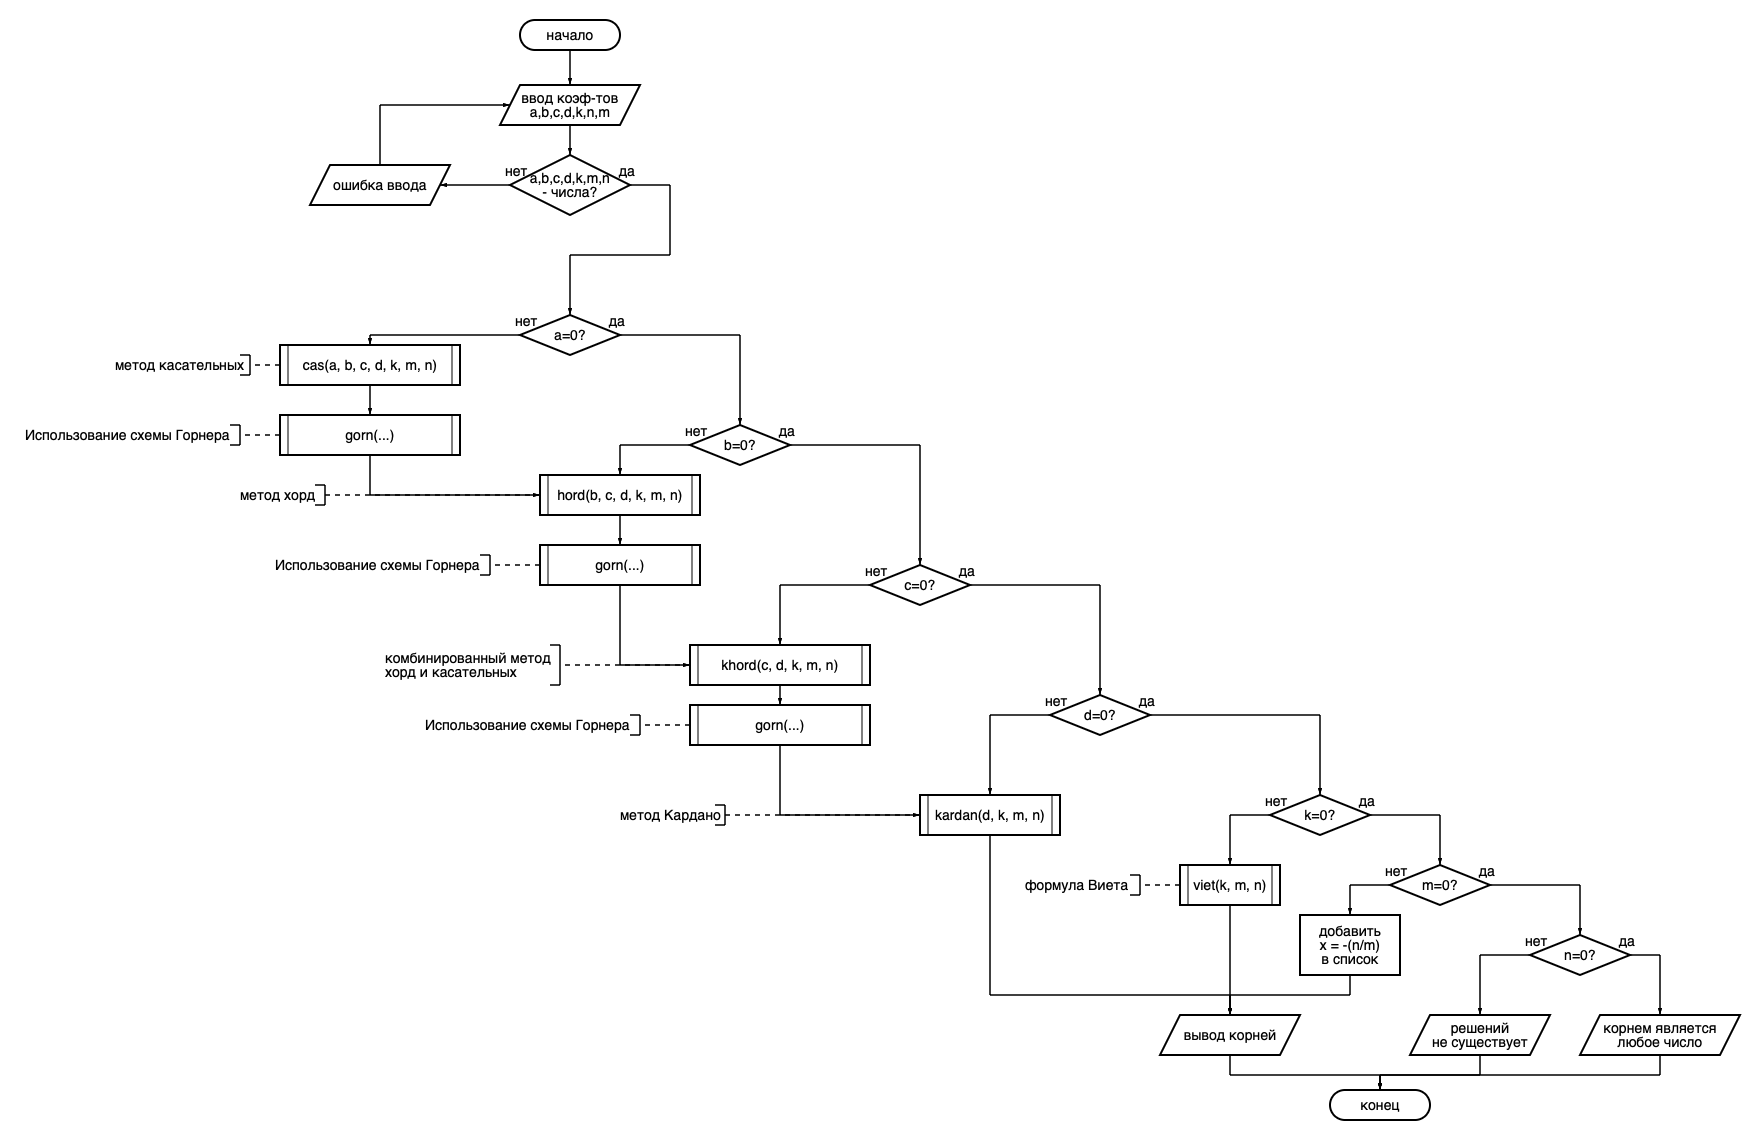
\includegraphics[width=0.95\textwidth]{All.png}
\caption{Главная программа}
\end{figure}

\begin{figure}[H]
\centering
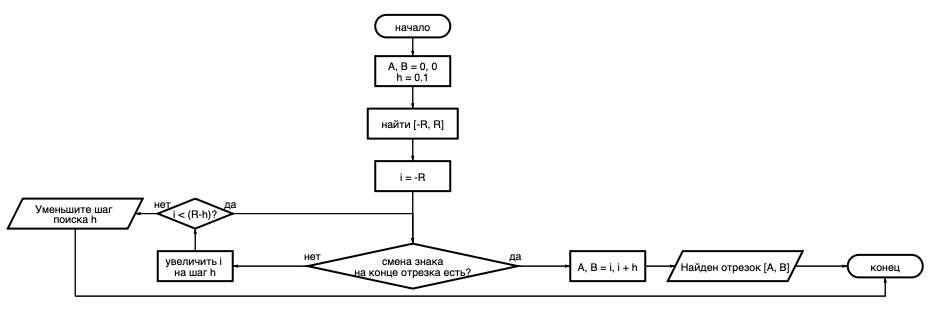
\includegraphics[width=0.85\textwidth]{otrez.png}
\caption{Поиск отрезка изоляции корня (findAB)}
\end{figure}

\begin{figure}[H]
\centering
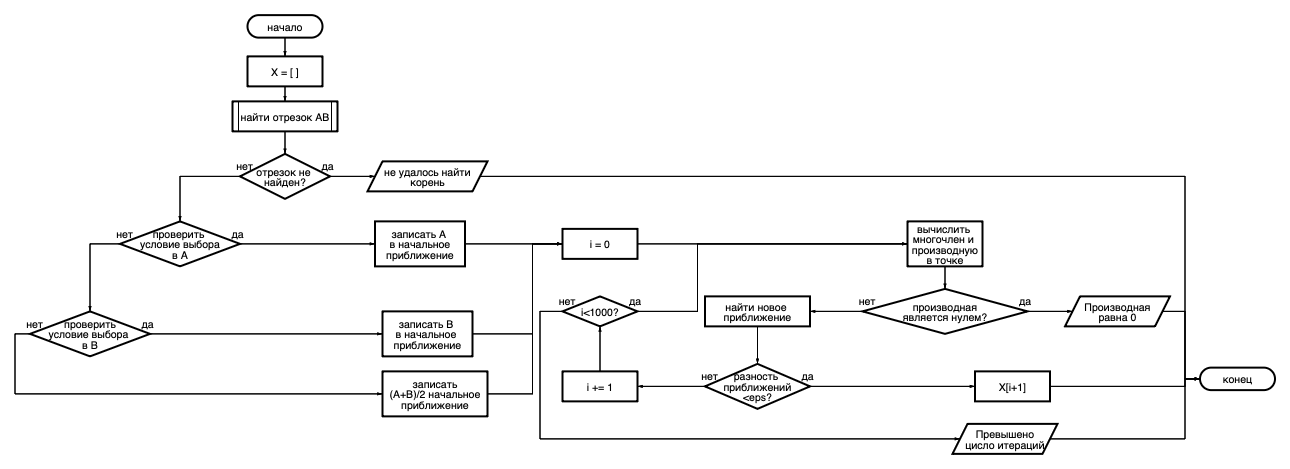
\includegraphics[width=0.85\textwidth]{casat.png}
\caption{Метод касательных (cas\_method)}
\end{figure}

\begin{figure}[H]
\centering
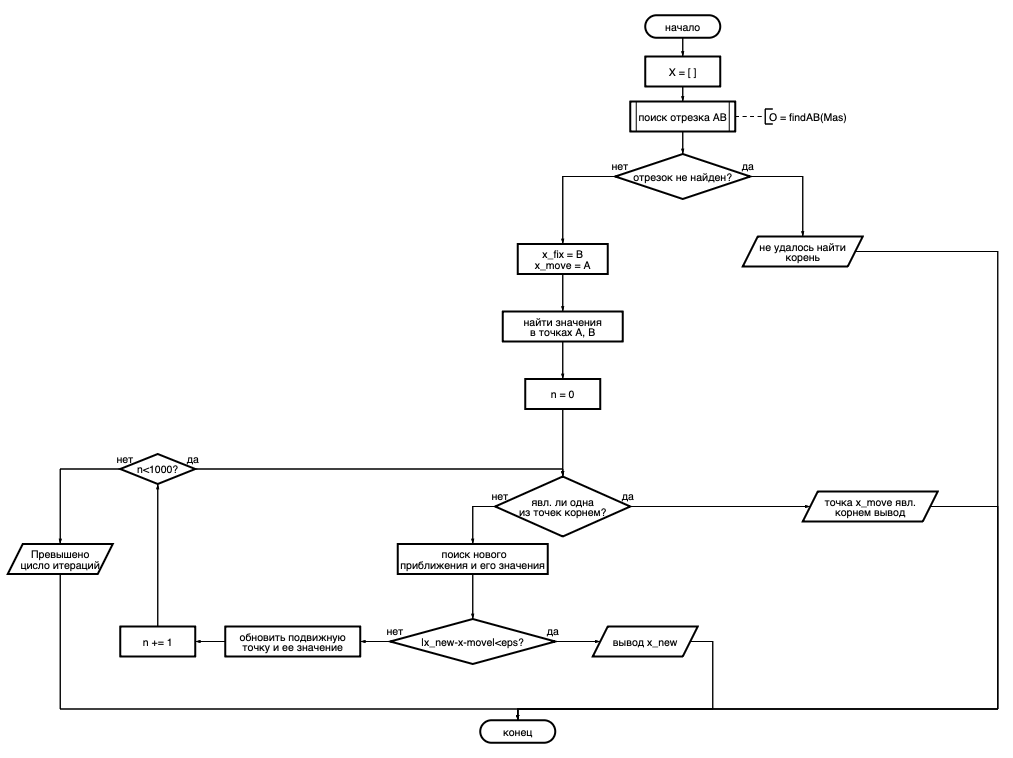
\includegraphics[width=0.85\textwidth]{hord.png}
\caption{Метод хорд (hord\_method)}
\end{figure}

\begin{figure}[H]
\centering
\includegraphics[width=0.85\textwidth]{combhord.png}
\caption{Комбинированный метод (khord\_method)}
\end{figure}

\begin{figure}[H]
\centering
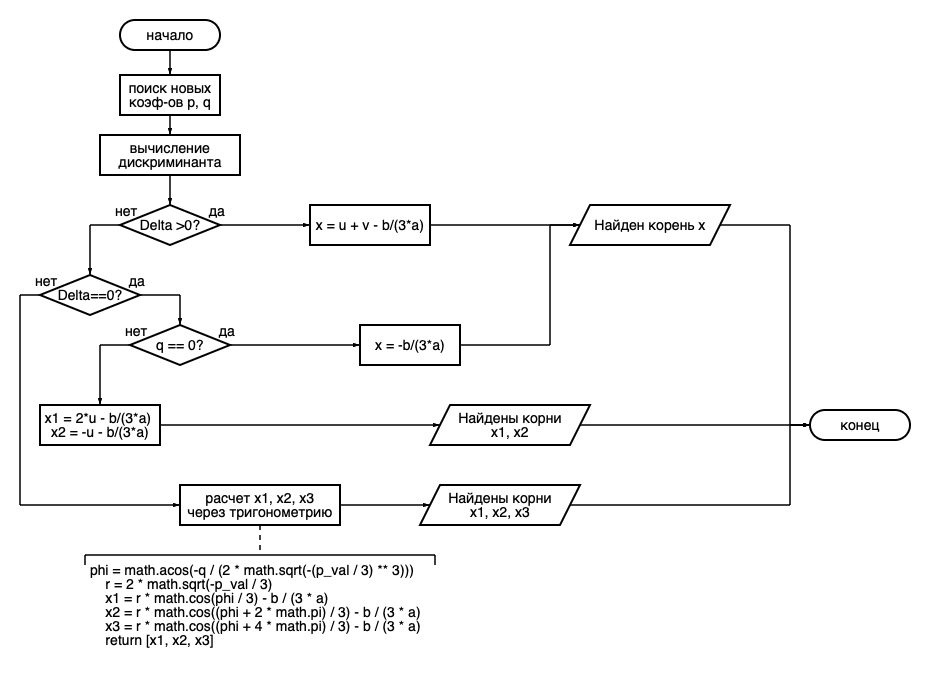
\includegraphics[width=0.85\textwidth]{cardan.png}
\caption{Метод Кардано (kardan)}
\end{figure}

\begin{figure}[H]
\centering
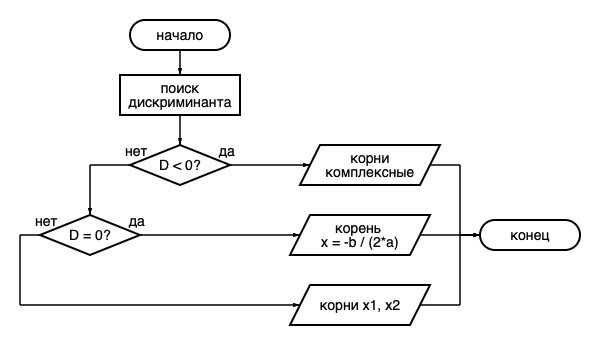
\includegraphics[width=0.85\textwidth]{viet.png}
\caption{Формулы Виета (viet)}
\end{figure}

\begin{figure}[H]
\centering
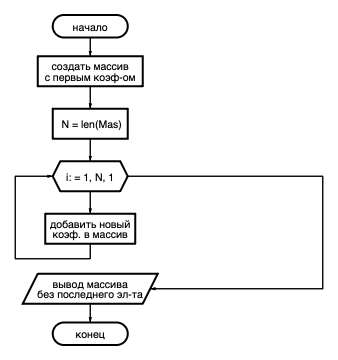
\includegraphics[width=0.85\textwidth]{gorn.png}
\caption{Схема Горнера (gorn)}
\end{figure}

\end{document}
